\section{Proposed Method}
\subsection{\revadd{Instance Segmentation With MSAM-Net}}
\subsubsection{Network Design}
To balance segmentation accuracy and computational efficiency, MSAM-Net uses YOLOv10 as the backbone and redesigns the segmentation head for baggage scenes. Baggage instances exhibit large scale variation, partial overlap, and fine boundary interference from tags and straps. MSAM-Net therefore contains two task-driven components: a four-level enhanced multi-branch feature pyramid network (4L-EMB-FPN) and an attention-guided multi-scale mask module (MSM). The architecture is shown in Fig.~\ref{fig:msam}.

\begin{figure*}[!t]
\centering
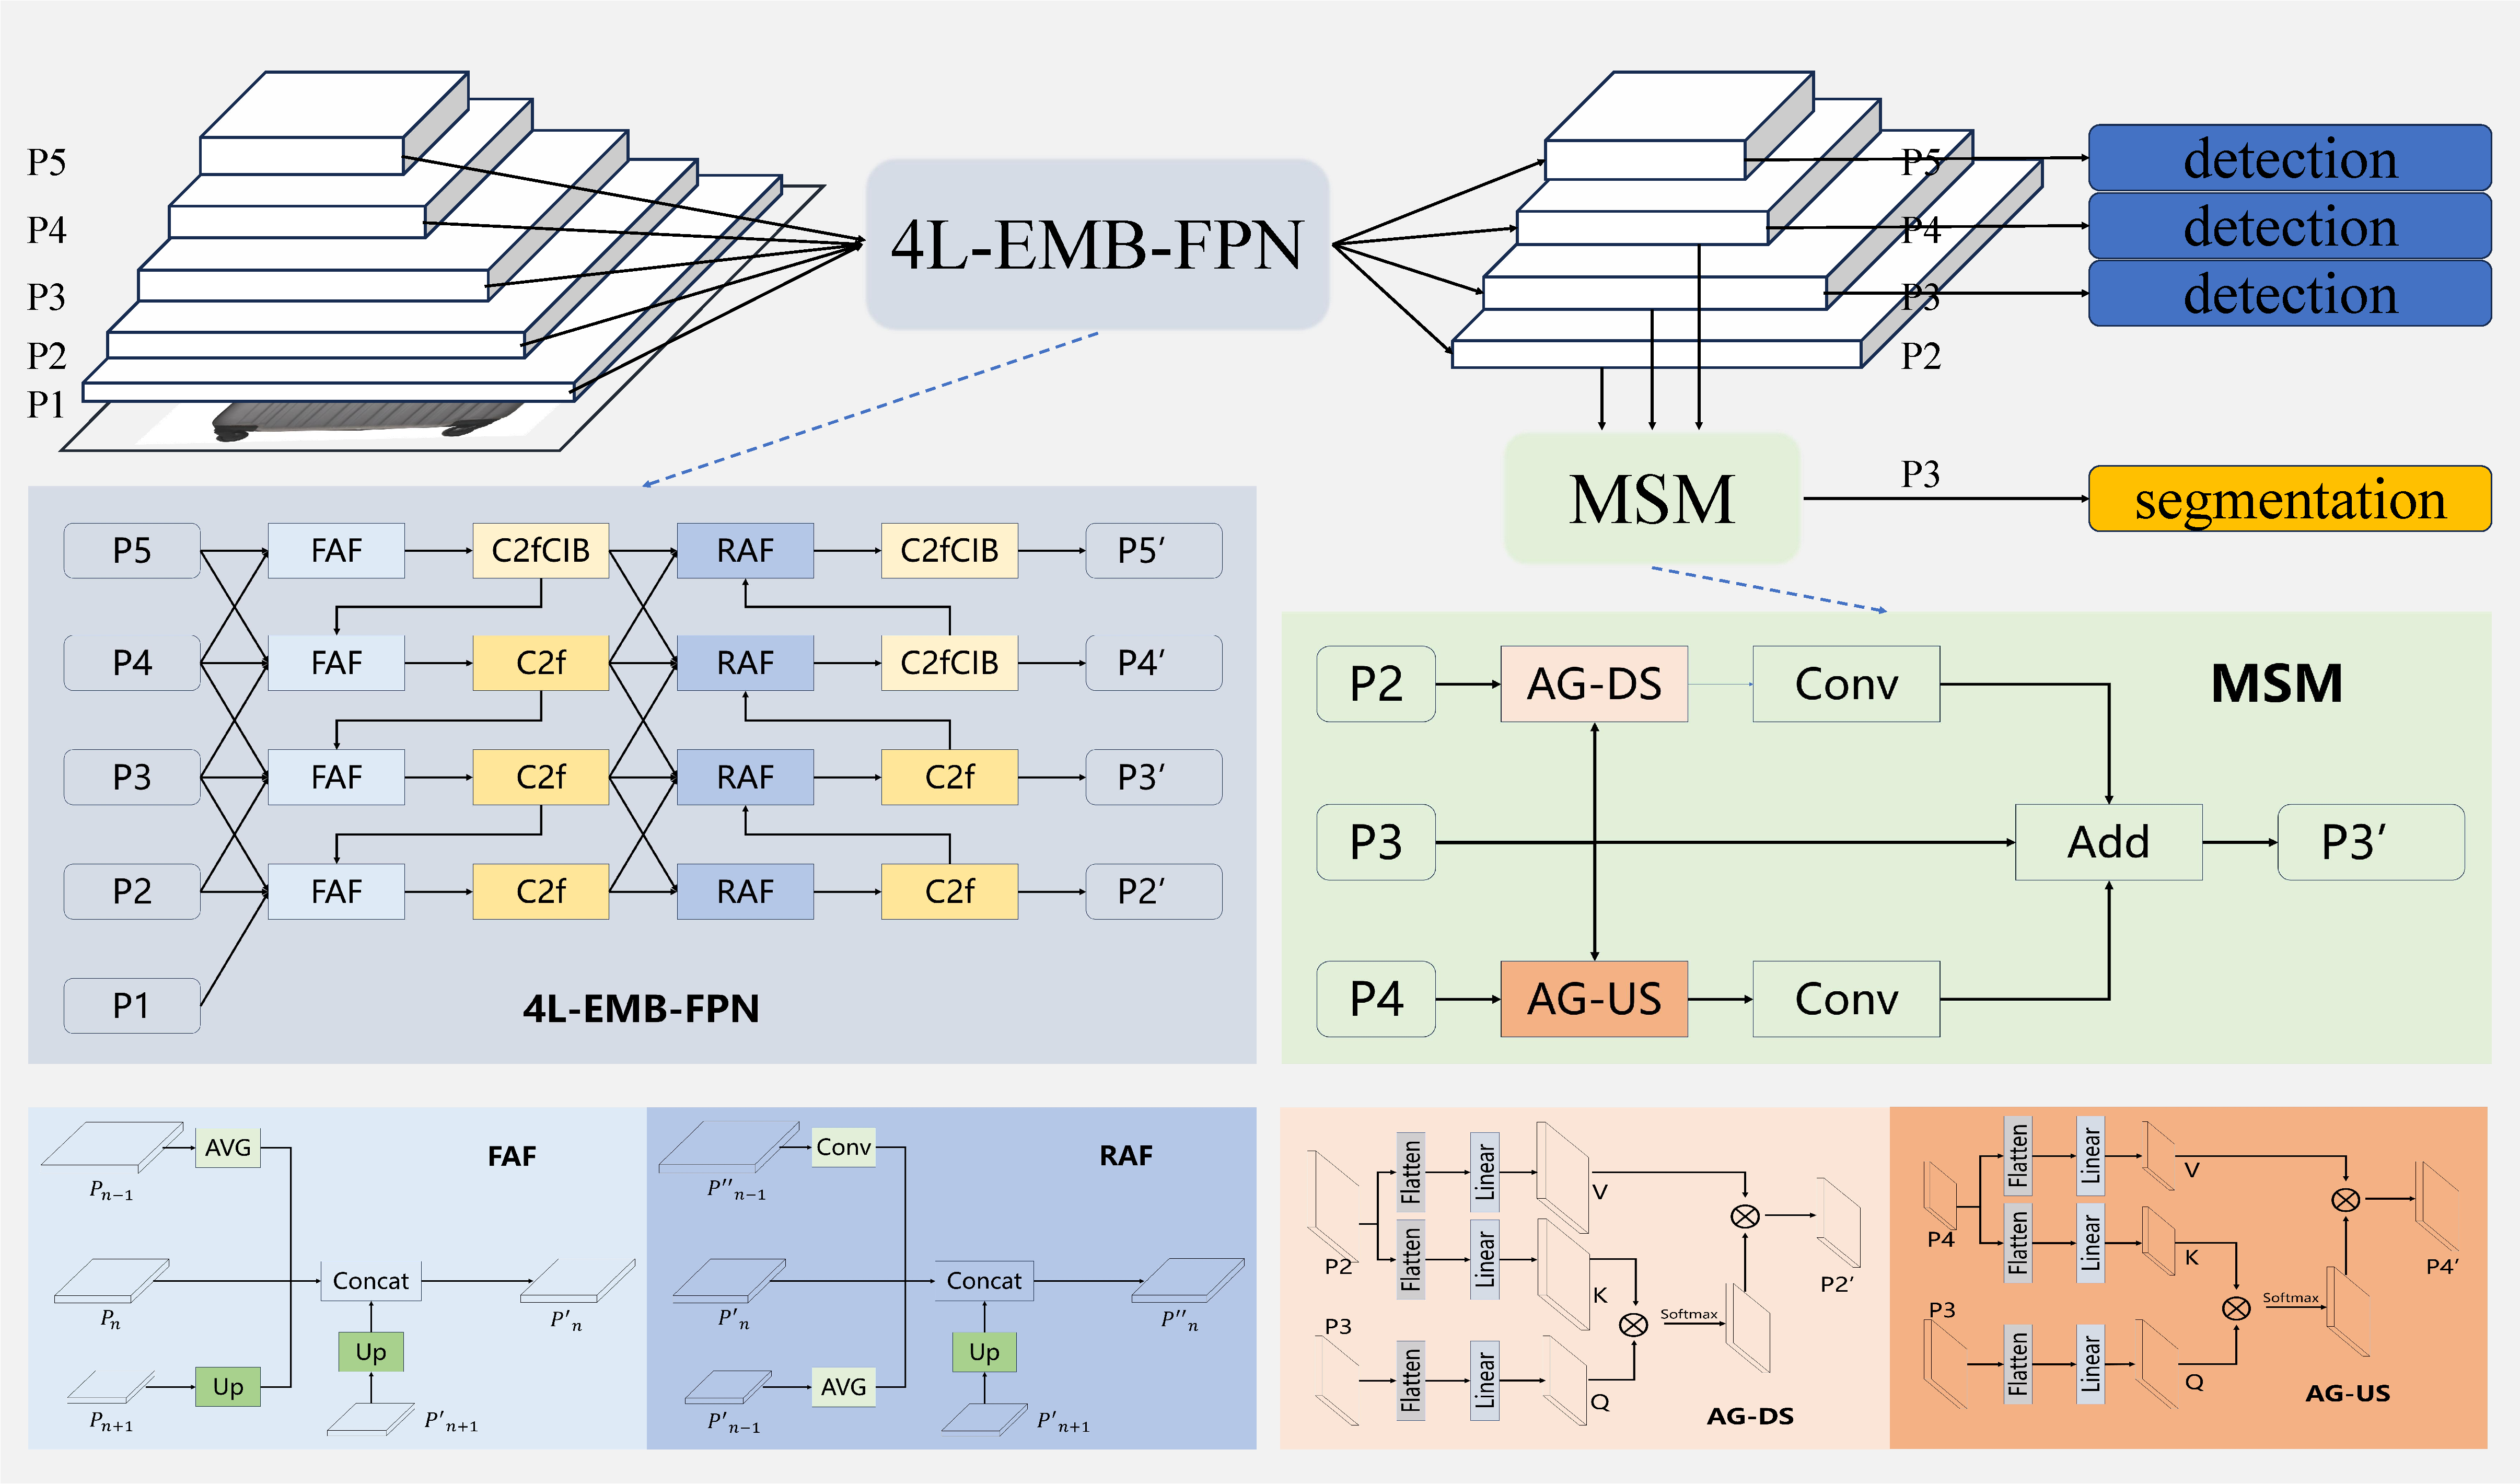
\includegraphics[width=0.9\textwidth]{figures/fig2.pdf}
\caption{Schematic overview of the proposed MSAM-Net architecture. \revadd{A YOLOv10 backbone is coupled with a four-level enhanced multi-branch feature pyramid (4L-EMB-FPN) for multi-scale feature aggregation and an attention-guided multi-scale mask module (MSM) for boundary refinement. MSM fuses $P_2$--$P_4$ features through attention-guided downsampling and upsampling to reduce tag and strap interference.}}
\label{fig:msam}
\end{figure*}

The 4L-EMB-FPN extracts four pyramid features, $P_2$--$P_5$, from the backbone. Low-level features preserve boundary details, whereas high-level features provide semantic context for large objects. To reduce semantic discrepancy between adjacent pyramid levels, a front-end aggregation fusion (FAF) module first aligns and fuses multi-level features. Given pyramid features $P_{n-1}$, $P_n$, $P_{n+1}$, and $P'_{n+1}$, where $P'_{n+1}$ denotes the refined feature at level $n+1$, FAF pools lower-level features, upsamples higher-level features, and concatenates them with $P_n$ to form an enriched representation $P'_n$. A refined aggregation fusion (RAF) module then further transforms, pools, upsamples, and concatenates these features to obtain $P''_n$. This two-stage fusion improves both large-instance semantic consistency and fine-grained boundary sensitivity.

\subsubsection{Attention-Guided Multi-Scale Mask Module}
Although the feature pyramid improves semantic representation, accurate mask reconstruction still requires explicit cross-scale interaction. The MSM uses $P_2$, $P_3$, and $P_4$ for mask prediction. Instead of using only interpolation or pooling, attention-guided downsampling (AG-DS) and attention-guided upsampling (AG-US) are used to exchange information between neighboring scales. In AG-DS, $P_3$ is projected as the query, while $P_2$ provides the key and value. In AG-US, $P_3$ is also used as the query, while $P_4$ provides the key and value. The attention operation is
\begin{equation}
\mathrm{Attention}(\boldsymbol{Q}_{x},\boldsymbol{K}_{y},\boldsymbol{V}_{y})=
\mathrm{Softmax}\left(\frac{\boldsymbol{Q}_{x}\boldsymbol{K}_{y}^{T}}{\sqrt{d}}\right)\boldsymbol{V}_{y},
\label{eq:attention}
\end{equation}
where $x\in\{\alpha,\beta\}$ indicates the downsampling or upsampling branch, $y\in\{2,4\}$ denotes the source pyramid level, and $d$ is the feature dimension. The attention outputs are reshaped and merged with the $P_3$ feature map.

To improve boundary regularity, an edge-aware mean-square error constraint is introduced using the distance field of the ground-truth boundary:
\begin{equation}
L_{\mathrm{MSE}}(\mathcal{B}_{\text{gt}},\mathcal{B}_{\text{pre}})=
\frac{1}{|\mathcal{B}_{\text{gt}}|}\sum_{\boldsymbol{p}\in\mathcal{B}_{\text{gt}}}d(\boldsymbol{p},\mathcal{B}_{\text{pre}})^{2},
\label{eq:mse}
\end{equation}
where $\mathcal{B}_{\text{gt}}$ and $\mathcal{B}_{\text{pre}}$ denote the ground-truth and predicted boundary-point sets, respectively, and $d(\boldsymbol{p},\mathcal{B}_{\text{pre}})$ is the shortest distance from point $\boldsymbol{p}$ to the predicted boundary.

\subsubsection{Training Objective}
The total loss combines standard detection losses with the segmentation constraint:
\begin{equation}
L_{\text{total}}=\lambda_{\text{box}}L_{\text{IOU}}+\lambda_{\text{seg}}L_{\text{seg}}+\lambda_{\text{cls}}L_{\text{cls}}+\lambda_{\text{dfl}}L_{\text{dfl}}.
\label{eq:loss}
\end{equation}
Here, $L_{\text{IOU}}$ is the CIoU-based box regression loss, $L_{\text{seg}}$ is the cropped mask reconstruction loss with the edge-aware boundary term, $L_{\text{cls}}$ is the BCE classification loss on task-aligned soft labels, and $L_{\text{dfl}}$ is the distribution focal loss for bounding-box localization. The weights $\lambda_{\text{box}}$, $\lambda_{\text{seg}}$, $\lambda_{\text{cls}}$, and $\lambda_{\text{dfl}}$ balance the four terms.

\begin{algorithm}[t]
\caption{Pixel-to-3D Cross Consistency Conditional Filtering (PX3C)}
\label{alg:px3c}
\begin{algorithmic}[1]

\Require Initial point cloud $P$ (masked by 2D results), thresholds
$\tau_{\mathrm{\text{thin}}},\tau_{\mathrm{\text{prot}}},\tau_{\mathrm{norm}}$

\Ensure Refined OBB $\mathrm{OBB}_{final}$, clean point set $P'$

\State \textbf{// Preprocessing Phase}

\State $P_{\text{down}} \gets \mathrm{VoxelGrid}(P)$
\State $P_{\text{rigid}} \gets \mathrm{RANSAC}(P_{\text{down}})$
    \Comment{Isolate luggage body}

\State $\mathrm{OBB}_{\text{cand}} \gets \mathrm{PCA}(P_{\text{rigid}})$
    \Comment{Initial candidate estimation}

\State $L_{\text{min}} \gets \mathrm{ShortestAxis}(\mathrm{OBB}_{\text{cand}})$

\State \revfix{Compute each point's distance to $\mathrm{OBB}_{\text{cand}}$ and remove the farthest $5\%$: $P_{\text{trim}} \gets \mathrm{Trim}_{0.05}(P_{\text{rigid}},\mathrm{OBB}_{\text{cand}})$.}

\State $P' \gets \emptyset$

\State \textbf{// Single-Pass Conditional Geometric Filtering}

\ForAll{$p_i \in P_{\text{trim}}$}

    \State Compute local neighborhood $\mathcal{N}(i)$,
           centroid $\bar{\boldsymbol p}$, and local normal $\boldsymbol n_i$

    \State \textbf{// Feature 1: Thin Slice}

    \State
    $f_{\text{thin}}=\frac{\max_{p\in\mathcal{N}(i)}\langle\boldsymbol{p}-\bar{\boldsymbol{p}},\boldsymbol{n}_i\rangle-
\min_{p\in\mathcal{N}(i)}\langle\boldsymbol{p}-\bar{\boldsymbol{p}},\boldsymbol{n}_i\rangle}{L_{\min}}$

    \State \textbf{// Feature 2: Protrusion}

    \State
    $d_{\text{out}}(i)
    \gets
    \mathrm{SignedDistance}
    \!\left(
    p_i,
    \mathrm{surface}(OBB_{\text{cand}})
    \right)$

    \State
    $f_{\text{prot}}
    \gets
    \max\!\left\{0,\,
    \frac{d_{\text{out}}(i)}{\epsilon_{\text{prot}}}
    \right\}$

    \State \textbf{// Feature 3: Normal Consistency}

    \State
    $f_{\text{norm}}
    \gets
    1-\left|\boldsymbol n_i\cdot\bar{\boldsymbol n}\right|$

    \State \textbf{// Filtering Condition: Remove if it matches tag/ribbon features}

    \If{$\neg \left(
            f_{\text{thin}}<\tau_{\text{thin}}
            \wedge
            f_{\text{prot}}>\tau_{\text{prot}}
            \wedge
            f_{\text{norm}}>\tau_{\text{norm}}
         \right)$}

        \State $P' \gets P' \cup \{p_i\}$
            \Comment{Keep points that are NOT tags/ribbons}

    \EndIf

\EndFor

\State \textbf{// Refined Reconstruction}

\State $\mathrm{OBB}_{\text{final}} \gets \mathrm{PCA}(P')$

\State \Return $\mathrm{OBB}_{\text{final}},\,P'$

\end{algorithmic}
\end{algorithm}

\subsection{\revadd{Spatio-Temporal Geometric Modeling}}
\subsubsection{PX3C Filtering}
Even after applying \revadd{the 2D mask from the instance segmentation module}, the projected point cloud often contains "ghost" points from unmasked ribbons or tag edges. To resolve this inconsistency between 2D segmentation and 3D geometry, we formulate the filtering process as a Conditional Geometric Self-Consistency problem. We employ standard preprocessing routines from the PCL, utilizing VoxelGrid downsampling for data regularization and RANSAC-based plane segmentation to isolate the rigid baggage body, and apply Principal Component Analysis (PCA) to construct the initial OBB $\mathcal{O}_{\text{cand}}$. \revadd{However, flexible attachments} can still distort standard PCA, causing the OBB to misalign (e.g., the main axis following a drifting ribbon). This creates a circular dependency: accurate filtering requires a reliable model, but the model itself depends on filtered data. We address this via a \revdel{self-bootstrapped conditional refinement that alternates between provisional model estimation and geometry-aware filtering} \revfix{single-pass self-bootstrapped refinement (Algorithm~\ref{alg:px3c}): one provisional OBB is estimated, a candidate-OBB trim is applied, and the retained points are filtered once before a final PCA reconstruction}.

\begin{algorithm}[t]
\caption{Consistency-Aware OBB Stabilization (CAOS)}
\label{alg:caos}
\begin{algorithmic}[1]

\Require Filtered point cloud $P_{\text{filt}}$,
current raw observation $b_t^{\text{raw}}$,
previous state $b_{t-1}$,
last stable snapshot $b^{*}$,
conveyor velocity $v$,
quality threshold $q_{\text{min}}$

\Ensure Stabilized OBB state $b_t$

\State \textbf{// Quality Assessment Phase}

\State
$C_{\text{main}}
\gets
\mathrm{EuclideanCluster}(P_{\text{filt}})$
\Comment{Largest connected component}

\State
$q_{\text{cov}}
\gets
\frac{|C_{\text{main}}|}{|P_{\text{filt}}|}$

\State
$q_{\text{in}}
\gets
\frac{
\left|
\left\{
p\in C_{\text{main}} :
d(p,O_t)\le \tau_{\text{in}}
\right\}
\right|
}
{|C_{\text{main}}|}
$

\State
\[
q_{\text{stab}}
\gets
\exp\!\left(
-\frac{
w_p\|\Delta P\|^2
+
w_r\|\Delta R\|^2
+
w_s\|\Delta S\|^2
}
{\eta}
\right)
\]

\State
$q
\gets
\alpha_1 q_{\text{cov}}
+
\alpha_2 q_{\text{in}}
+
\alpha_3 q_{\text{stab}}$

\State \textbf{// Adaptive Smoothing Weight}

\State
$\beta(q)
\gets
\min\!\left(
\beta_{\text{max}},
k(1-q)
\right)$

\State \textbf{// Dynamic State Update Strategy}

\If{$q<q_{\text{min}}$}

    \State \textbf{// Low Quality: Extrapolate from Last Stable State}

    \State
    $\Delta t_{\text{gap}}
    \gets
    \mathrm{TimeSince}(b^{*})$

    \State
    $b_t
    \gets
    b^{*}
    \oplus
    \left(v\cdot\Delta t_{\text{gap}}\right)$

\Else

    \State \textbf{// High Quality: Adaptive Smoothing}

    \State \revfix{Linearly interpolate position and size; update orientation with quaternion SLERP.}

    \State
    \[
    b_t
    \gets
    \left(1-\beta(q)\right)b_t^{\text{raw}}
    +
    \beta(q)
    \left(
    b_{t-1}
    \oplus
    (v\cdot\Delta t)
    \right)
    \]

    \State
    $b^{*} \gets b_t$
    \Comment{Update reference snapshot}

\EndIf

\State \Return $b_t$

\end{algorithmic}
\end{algorithm}

\begin{figure}[!t]
\centering
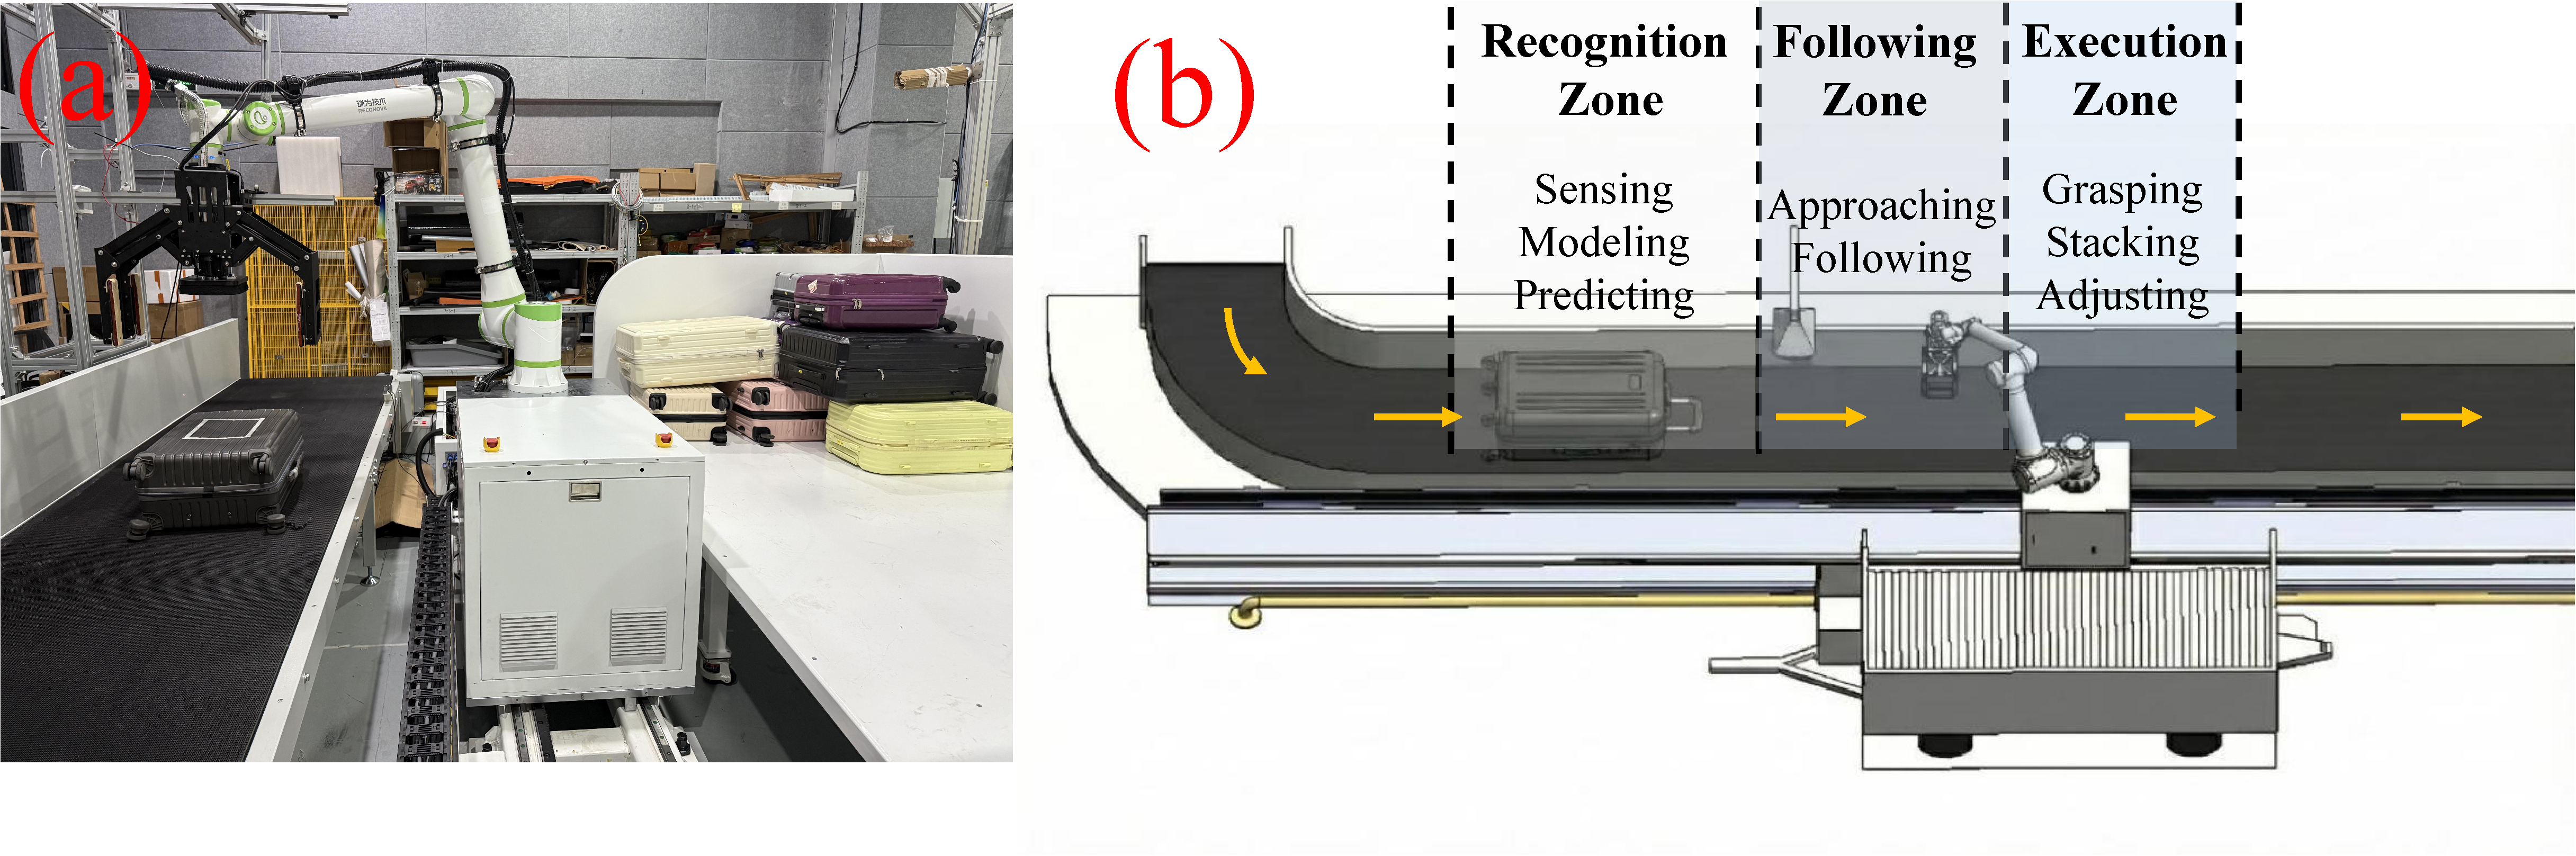
\includegraphics[width=\columnwidth]{figures/fig3_rev.pdf}
\caption{(a) Hardware platform. (b) System Workflow of the \revadd{Dynamic Grasping Strategy.}}
\label{fig:planning}
\end{figure}

For each point $P_i$, three features are computed. The thin-slice feature evaluates the local thickness relative to the shortest OBB dimension $L_{\min}$:
\begin{equation}
f_{\text{thin}}=\frac{\max_{p\in\mathcal{N}(i)}\langle\boldsymbol{p}-\bar{\boldsymbol{p}},\boldsymbol{n}_i\rangle-
\min_{p\in\mathcal{N}(i)}\langle\boldsymbol{p}-\bar{\boldsymbol{p}},\boldsymbol{n}_i\rangle}{L_{\min}},
\label{eq:fthin}
\end{equation}
where $\mathcal{N}(i)$ is the local neighborhood, $\bar{\boldsymbol{p}}$ is the neighborhood centroid, $\boldsymbol{n}_i$ is the local normal at $P_i$, and $\bar{\boldsymbol n}$ is the dominant rigid-body normal. The protrusion feature measures the normalized distance outside the OBB:
\begin{equation}
f_{\text{\text{prot}}}=\max\{0,d_{\text{\text{out}}}(i)/\epsilon_{\text{\text{prot}}}\},
\label{eq:fprot}
\end{equation}
where $d_{\text{out}}(i)$ is the signed distance to the OBB surface. The normal-consistency feature is
\begin{equation}
f_{\text{norm}}=1-|\boldsymbol{n}_{i}\cdot\bar{\boldsymbol{n}}|,
\label{eq:fnorm}
\end{equation}
where $\boldsymbol{n}_{i}$ is the local normal and $\bar{\boldsymbol{n}}$ is the dominant rigid-body surface normal. Points satisfying the combined flexible-interference condition are removed, and PCA is applied again to reconstruct the refined OBB. \revfix{This single-pass self-bootstrapped refinement reduces the effect of residual 2D segmentation leakage and produces a rigid-body representation more suitable for grasp planning.}

\subsubsection{CAOS Temporal Stabilization}
Single-frame OBB estimates may still fluctuate because of motion blur, occlusion, or depth noise. To prevent erratic control commands, we employ the CAOS method (see Algorithm~\ref{alg:caos}), which utilizes multi-frame consistency for stabilization. CAOS stabilizes the OBB sequence using quality-aware temporal smoothing. \revfix{Here $\boldsymbol n_i$ and $\bar{\boldsymbol n}$ denote the local and dominant body normals, respectively; $\mathcal{O}_t$ is the current OBB; and $\Delta\boldsymbol P$, $\Delta\boldsymbol R$, and $\Delta\boldsymbol S$ denote frame-to-frame changes in position, rotation, and size. The operator $\boldsymbol b\oplus(\boldsymbol v\Delta t)$ translates position only.} Let $\mathcal{P}_{\text{filt}}$ be the filtered point cloud and $\mathcal{C}_{\text{main}}\subseteq\mathcal{P}_{\text{filt}}$ be the largest connected component. The coverage score and inlier-rate score are defined as
\begin{equation}
q_{\text{cov}}=\frac{|\mathcal{C}_{\text{\text{main}}}|}{|\mathcal{P}_{\text{\text{filt}}}|},\quad
q_{\text{in}}=\frac{\left|\{p\in\mathcal{C}_{\text{\text{main}}}:d(p,\mathcal{O}_{t})\le\tau_{\text{\text{in}}}\}\right|}{|\mathcal{C}_{\text{\text{main}}}|}.
\label{eq:qcov}
\end{equation}
The first score measures whether the point cloud is dominated by one coherent object, while the second measures how well the estimated OBB fits the observed points. Temporal stability is quantified as
\begin{equation}
q_{\text{\text{stab}}}=\exp\left(-\frac{w_p\|\Delta\boldsymbol{P}\|^2+w_r\|\Delta\boldsymbol{R}\|^2+w_s\|\Delta\boldsymbol{S}\|^2}{\eta}\right),
\label{eq:qstab}
\end{equation}
where $\Delta\boldsymbol{P}$, $\Delta\boldsymbol{R}$, and $\Delta\boldsymbol{S}$ denote changes in position, rotation, and scale. The aggregate quality score is written as:
\begin{equation}
q=\alpha_1q_{\text{cov}}+\alpha_2q_{\text{\text{in}}}+\alpha_3q_{\text{\text{stab}}}.
\end{equation}
and the output OBB state is updated by:
\begin{equation}
\boldsymbol{b}_{t}=\begin{cases}
\boldsymbol{b}^{*}\oplus(\boldsymbol{v}\Delta t_{\text{gap}}), & q<q_{\text{min}},\\
(1-\beta(q))\boldsymbol{b}_{t}^{\text{raw}}+\beta(q)(\boldsymbol{b}_{t-1}\oplus(\boldsymbol{v}\Delta t)), & \mathrm{otherwise},
\end{cases}
\label{eq:caos}
\end{equation}
where $\boldsymbol{b}^{*}$ is the last reliable snapshot, $\boldsymbol{b}_{t}^{\text{raw}}$ is the current PX3C observation, $\oplus(\boldsymbol{v}\Delta t)$ denotes conveyor-motion compensation over duration $\Delta t$, and $\beta(q)=\min(\beta_{\text{max}},k(1-q))$ is an adaptive smoothing coefficient. \revfix{The position and size components use linear interpolation, while orientation uses quaternion SLERP.} \revadd{$q_{\text{cov}}$, $q_{\text{in}}$, and $q_{\text{stab}}$ denote coverage, inlier rate, and temporal stability, respectively, and $q$ is their weighted quality score.} A lower quality score increases the reliance on historical prediction, thereby preventing abrupt and unreliable control commands.

\begin{figure}[!t]
\centering
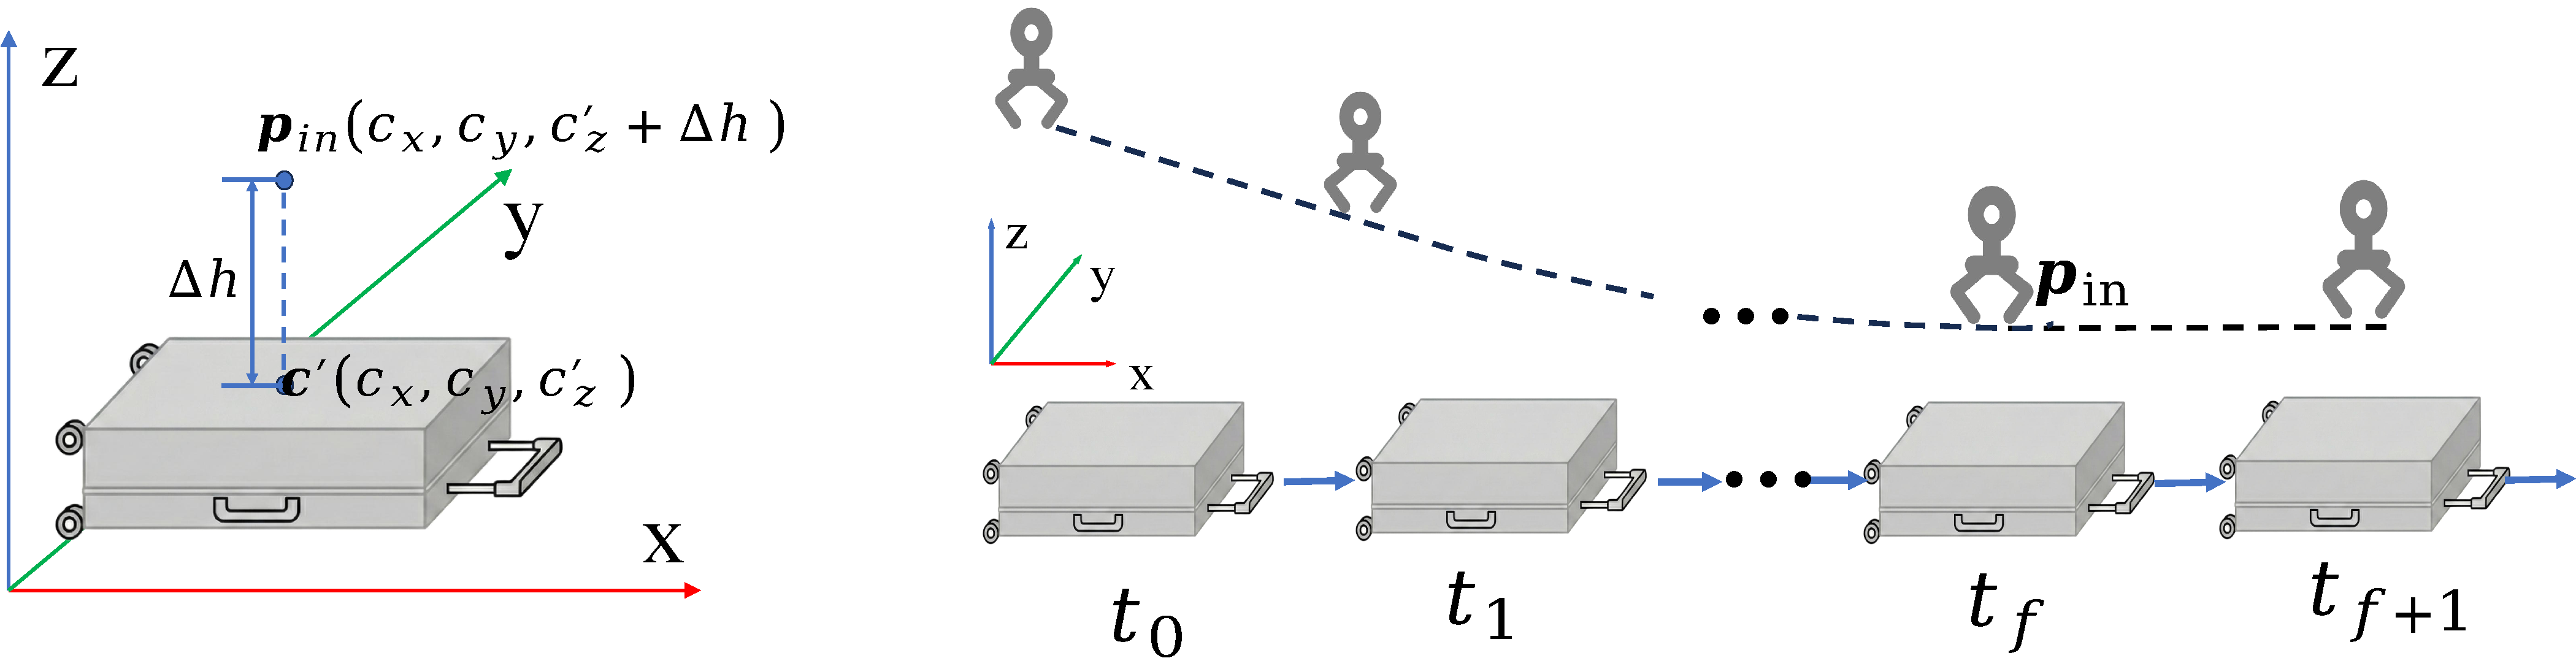
\includegraphics[width=\columnwidth]{figures/fig4.pdf}
\caption{Diagram of the Interception Point $P_{\text{\text{in}}}$ and Rapid Interception Strategy.}
\label{fig:rapid_interception}
\end{figure}

\subsection{\revadd{Dynamic Grasping and Active State Regulation}}
We adopt a "Predict-Follow-Grasp" execution paradigm, as illustrated in Fig. \ref{fig:planning}. The process involves visual perception and modeling in the Recognition Zone, followed by velocity synchronization in the Following Zone, and finally, grasping execution in the Execution Zone.
\subsubsection{Recursive Bayesian State Estimation}
The dynamic state of the baggage centroid is estimated using a discrete Kalman filter with a constant-acceleration model. The state vector is
\begin{equation}
\boldsymbol{x}_{k}=[p_x,v_x,a_x,p_y,v_y,a_y,p_z,v_z,a_z]^T.
\end{equation}
The process and observation models are
\begin{equation}
\begin{cases}
\boldsymbol{x}_{k}=\boldsymbol{F}\boldsymbol{x}_{k-1}+\boldsymbol{w}_{k-1},\\
\boldsymbol{z}_{k}=\boldsymbol{H}\boldsymbol{x}_{k}+\boldsymbol{v}_{k},
\end{cases}
\label{eq:state}
\end{equation}
where $\boldsymbol{z}_{k}$ is the observed centroid, $\boldsymbol{w}_{k-1}\sim\mathcal{N}(0,\boldsymbol{Q})$ is the process noise, and $\boldsymbol{v}_{k}\sim\mathcal{N}(0,\boldsymbol{R})$ is the measurement noise. \revfix{The observation relation is $\boldsymbol{H}\boldsymbol{x}_{k}=[p_x,p_y,p_z]^{T}$.} The transition matrix is block diagonal:
\begin{equation}
\boldsymbol{F}=\mathrm{diag}(\boldsymbol{F}_{x},\boldsymbol{F}_{y},\boldsymbol{F}_{z}),
\end{equation}
with
\begin{equation}
\boldsymbol{F}_{x}=\revaddmath{\boldsymbol{F}_{y}=\boldsymbol{F}_{z}=}\begin{bmatrix}
1 & \Delta T & \frac{1}{2}\Delta T^{2}\\
0 & 1 & \Delta T\\
0 & 0 & 1
\end{bmatrix}.
\label{eq:fx}
\end{equation}

The filter operates in a \textit{Predict-Update} cycle. \revadd{The prior and posterior state estimates are $\hat{\boldsymbol{x}}_k^{-}$ and $\hat{\boldsymbol{x}}_k$, with error covariances $\boldsymbol{P}_k^{-}$ and $\boldsymbol{P}_k$, respectively.} In the \textit{Predict} phase, we extrapolate the prior state $\hat{\boldsymbol{x}}_{k}^{-}$ and the error covariance $\boldsymbol{P}_{k}^{-}$ based on the optimal estimation \revadd{$\hat{\boldsymbol{x}}_{k-1}$} from the previous step:
\begin{equation}
\hat{\boldsymbol{x}}_{k}^{-}=\boldsymbol{F}\hat{\boldsymbol{x}}_{k-1},\
\boldsymbol{P}_{k}^{-}=\boldsymbol{F}\boldsymbol{P}_{k-1}\boldsymbol{F}^{T}+\boldsymbol{Q},
\label{eq:kf_predict}
\end{equation}
and in the \textit{Update} phase, the Kalman Gain $\boldsymbol{K}_{k}$ is computed using the current observation $\boldsymbol{z}_k$ to correct the prior error, yielding \revadd{the posterior estimate $\hat{\boldsymbol{x}}_k$} and the updated posterior error covariance $\boldsymbol{P}_{k}$ as:
\begin{equation}
\begin{cases}
    \boldsymbol{K}_{k}=\boldsymbol{P}_{k}^{-}\boldsymbol{H}^{T}(\boldsymbol{H}\boldsymbol{P}_{k}^{-}\boldsymbol{H}^{T}+\boldsymbol{R})^{-1}, \\
\hat{\boldsymbol{x}}_{k}=\hat{\boldsymbol{x}}_{k}^{-}+\boldsymbol{K}_{k}(\boldsymbol{z}_{k}-\boldsymbol{H}\hat{\boldsymbol{x}}_{k}^{-}), \\
\boldsymbol{P}_{k}=(\boldsymbol{I}-\boldsymbol{K}_{k}\boldsymbol{H})\boldsymbol{P}_{k}^{-}.
\end{cases}
\end{equation}
The trace of $\boldsymbol{P}_{k}$ is used as an uncertainty indicator. When collision, sliding, or occlusion causes the observation model to fail, the uncertainty increases and can trigger active state regulation. This serves as a robust metric to determine whether the target is maintaining stable motion. 

For rotation prediction, since rotation on conveyor belts is typically gradual, we apply the same smoothing filter as the position estimation to the components of the quaternion $\boldsymbol{q}_t$. The target position for a future timestamp $t_p$ is computed as:
\begin{equation}
\boldsymbol{c}(t_p)=\hat{\boldsymbol{p}}_{\text{now}}+\hat{\boldsymbol{v}}_{\text{now}}(t_p-t_{\text{now}})+\frac{1}{2}\hat{\boldsymbol{a}}_{\text{now}}(t_p-t_{\text{now}})^2.
\end{equation}
Quaternion components $\boldsymbol{q}(t_p)$ are normalized before conversion to the rotation matrix with $\boldsymbol{R}(t_p) = \mathrm{quat2rot}(\frac{\boldsymbol{q}(t_p)}{\left \| \boldsymbol{q}(t_p) \right \| })$ for the robot controller.

\subsubsection{Coarse-to-Fine Planning in Relative Velocity Space}
The grasping planner contains two stages, as shown in Algorithm~\ref{algo:two_stage_dynamic_grasping}. \revfix{We take the current planning instant as $t_0$ and use $\boldsymbol{P}_{\text{start}}=\boldsymbol{p}_{\text{EE}}(t_0)$ for the end-effector position.} Stage I performs rapid interception. The end-effector moves toward an interception point above the predicted target trajectory in minimal time. \revfix{Let $\boldsymbol{p}_{\text{obj}}(t)$ denote the target position predicted by the state estimator for $t\ge t_0$.} Rather than solving a full dynamic trajectory optimization problem, the earliest interception time $t_f$ is estimated from
\begin{equation}
\|\boldsymbol{p}_{\text{obj}}(t_f)-\boldsymbol{P}_{\text{start}}\|-\revfixmath{\bar v}(t_f-t_0)=0,
\label{eq:interception}
\end{equation}
where \revfix{$\bar v$} is the average feasible robot velocity. \eqref{eq:interception} is solved using Newton--Raphson updates. To compensate for neglected acceleration and jerk constraints, a buffer term is added:
\begin{equation}
t_{\text{inter}}=t_f+\Delta t_{\text{buffer}},\quad
\Delta t_{\text{buffer}}=\alpha\frac{v_{\text{max}}}{a_{\text{max}}}, \label{equ:estimate}
\end{equation}
where $\alpha$ is a safety factor set to 1.2. \revfix{The offset point used for execution is then $\boldsymbol{P}_{\text{in}}=\boldsymbol{p}_{\text{obj}}(t_{\text{inter}})+[0,0,\Delta h]^T$; it is the target position predicted at the buffered interception time, rather than the current position.}

Stage II performs fine synchronization in relative velocity space. The dynamic grasping task is converted into a relative alignment problem by minimizing
\begin{equation}
E_{\text{sync}}(t)=\frac{\|\boldsymbol{v}_{\text{EE}}(t)-\boldsymbol{v}_{\text{obj}}(t)\|^2}{v_{\text{ref}}^{2}}+
\lambda\frac{\|\boldsymbol{p}_{\text{EE}}^{xy}(t)-\boldsymbol{p}_{\text{obj}}^{xy}(t)\|^2}{d_{\text{ref}}^{2}}.
\label{eq:sync}
\end{equation}
\revfix{Here $\boldsymbol{v}_{\text{obj}}(t)$ is the predicted conveyor/object velocity of the target, and the position term uses the same target trajectory.} The first term measures velocity synchronization, and the second term measures planar position alignment. When $E_{\text{sync}}<\epsilon_{\text{safe}}$, the end-effector and target are treated as relatively static, and the robot performs the final short vertical descent. \revdel{Because the descent distance is only 80~$\mathrm{mm}$, the residual relative velocity is negligible during this interval.} \revfix{The descent distance is $\Delta h=80~\mathrm{mm}$ and is executed at $v_z=0.20~\mathrm{m/s}$ ($T_{\text{desc}}=0.40~\mathrm{s}$); horizontal compensation continues using $\boldsymbol{v}_{\text{obj}}(t)$ throughout the descent.} The final motion is therefore planned as a local point-to-point trajectory using a quintic polynomial.

\revdel{The earlier algorithm mixed $p(t)$ with $p_{\mathrm{obj}}(t)$, $p_{\mathrm{start}}$ with $P_{\mathrm{start}}$, and $t_f$ with $t_{\mathrm{inter}}$, and it omitted the time origin.} \revfix{Algorithm~\ref{algo:two_stage_dynamic_grasping} uses $t_0$ as the time origin and uses $\boldsymbol{p}_{\mathrm{obj}}(t)$, $\boldsymbol{P}_{\mathrm{start}}$, and $t_{\mathrm{inter}}$ consistently.}

\begin{algorithm}[t]
\caption{Two-Stage Dynamic Grasping Planning Strategy}
\label{algo:two_stage_dynamic_grasping}
\begin{algorithmic}[1]

\Require Target state estimate
$\hat{\mathbf{x}}_k=
[\mathbf{p}_{\text{obj}},\mathbf{v}_{\text{obj}}]^{T}$;
robot kinematic limits $v_{\text{max}},a_{\text{max}}$;
thresholds $\epsilon_{\text{safe}},\lambda,v_{\text{ref}},d_{\text{ref}}$

\Ensure Robot position command vector $\mathbf{q}_{\text{cmd}}$

\State \textbf{// Stage 1: Fast Interception (Coarse Planning)}

\State Define interception offset point
$P_{\text{in}}=\mathbf{p}_{\text{obj}}+[0,0,\Delta h]^{T}$

\State Initialize $t_f$ using heuristic estimation

\Repeat

    \State Update $t_f$ using Newton--Raphson on distance constraint:

    \State
    $f(t)=
    \left\|
    \mathbf{p}_{\text{obj}}(t)-P_{\text{start}}
    \right\|
    -
    v_{\text{avg}}\cdot t$

\Until{convergence}

\State Apply buffer term:
$t_{\text{inter}}\gets t_f+\alpha\frac{v_{\text{max}}}{a_{\text{max}}}$

\State Execute trajectory to reach $P_{\text{in}}$ at time $t_{\text{inter}}$

\State \textbf{// Stage 2: Synchronization (Relative Velocity Space)}

\While{grasp not completed}

    \State Obtain real-time error vectors
    $\mathbf{v}_{\text{err}},\mathbf{p}_{\text{err}}$

    \State Compute normalized synchronization cost $E_{\text{sync}}$:

    \State
    $E_{\text{sync}}
    \gets
    \frac{\left\|\mathbf{v}_{\text{err}}\right\|^2}{v_{\text{ref}}^{2}}
    +
    \lambda
    \frac{\left\|\mathbf{p}_{\text{err}}\right\|^2}{d_{\text{ref}}^{2}}$

    \If{$E_{\text{sync}}<\epsilon_{\text{safe}}$}
        \Comment{Condition met: relative static state}

        \State Trigger Z-axis descent to target surface

        \State Close gripper

        \State \Return success

    \Else

        \State Compute control input to minimize $E_{\text{sync}}$

        \State Update $\mathbf{q}_{\text{cmd}}$ via inverse kinematics

    \EndIf

\EndWhile

\end{algorithmic}
\end{algorithm}

\subsubsection{Active State Regulation}
\revfix{A weakly coupled pipeline would pass an unreliable geometric state directly to execution. Our physical feedback loop instead uses uncertainty or synchronization failure to trigger suction relocation, which changes the baggage configuration; the system then re-acquires RGB-D observations, re-estimates the state, and replans the grasp.}
Passive visual servoing assumes that observation uncertainty will eventually decrease as additional frames are received. This assumption is not always valid in conveyor-belt baggage handling.  \revadd{Stacked or colliding objects may remain poorly observable or prevent synchronization. Such configurations can lead to high-entropy object states and increased control uncertainty.}  \revadd{The proposed active state-regulation mechanism} addresses this failure mode by allowing the robot to reshape the environment.  \revadd{When $\mathrm{tr}(\boldsymbol{P}_{p,k})>\tau_P$ or $E_{\text{sync}}$ does not converge, precision placement is temporarily aborted. Here, $\boldsymbol{P}_{p,k}$ is the covariance submatrix for $[p_x,p_y,p_z]^T$. We set $\tau_P=4.0\times10^{-4}~\mathrm{m}^2$, corresponding to a root-sum-of-variances positional uncertainty of 0.020~$\mathrm{m}$.} The robot then performs a best-effort suction grasp based on the predicted centroid and relocates the baggage to an empty conveyor region detected by the vision system. This reset action converts a chaotic or poorly observable state into an ordered state for subsequent handling, thereby closing the loop between perception and manipulation. \revadd{After relocation, the system acquires new RGB-D observations, re-estimates the target state, and replans normal gripper-based grasping.}
